\documentclass[12pt]{article}

% packages
\usepackage{graphicx}
\usepackage{afterpage}
\usepackage[T1]{fontenc}
\usepackage{afterpage}
\usepackage{amsmath,bm}
\usepackage{amsthm}
\usepackage{parskip}
\usepackage{minted}
\usepackage{amsfonts}
\usepackage[hidelinks]{hyperref}
\usepackage[backend=biber]{biblatex} 
 
% commands
\newcommand\blankpage{%
    \null%
    \thispagestyle{empty}%
    \addtocounter{page}{-1}%
    \newpage%
}

% cambio del nome alla tabella dei contenuti
\renewcommand*\contentsname{Indice}

% graphic settings
\graphicspath{ {./images/} }

% thm definitions
\theoremstyle{definition}
\newtheorem*{esempio}{Esempio}

% risorse bibliografia (run "biber main" to compile)
\addbibresource{bibliography.bib}

\begin{document}

    % prima pagina
    \begin{titlepage}
    \begin{center}
        
        \includegraphics*[width=0.8\linewidth]{universita_degli_studi_di_genova.png}
        
        \vspace*{0.5cm}

        \textbf{Dipartimento di Informatica, Bioingegneria, Robotica e Ingegneria dei Sistemi}

        \vspace*{0.5cm}

        \textbf{Corso di Laurea Triennale in Informatica}\\
        \textbf{Anno Accademico} 2021/2022

        \vspace*{2cm}
        
        \LARGE
        \textbf{Analisi di serie temporali\\\large Aspetti Applicativi}

        \vspace*{5.5cm}

        \normalsize

        \textit{Candidato}
        \hfill
        \textit{Relatore}\\

        Alex Valle
        \hfill
        Prof.\ Francesca Odone\\

    \end{center}
\end{titlepage}

    % indice
    \tableofcontents

    % introduzione
    \section{Introduzione}
In tale capitolo introduttivo verranno spiegati gli obbiettivi e la suddivisione del tirocinio
in merito al tempo disponibile, cercando di spiegare, in maniera sintetica, come è stato
svolto ed organizzato.

\subsection{Premessa}
Lo scopo di questo elaborato è quello di descrivere l'esperienza di tirocinio svoltasi presso
l'Università Degli Studi di Genova con durata complessiva di 300 ore con inizio 25 novembre 2022
e fine 27 febbraio 2023. Il tirocinio è stato svolto per la maggior parte del tempo da remoto
con incontri, volti all'andamento di esso, mediante l'utilizzo di Teams (piattaforma sviluppata da Microsoft)
che in presenza presso il dipartimento. 

\subsection{Obbiettivi}
L'obbiettivo di questo tirocinio è stato quello di provare a individuare, se esistenti, uno o più metodi, 
relativi all'analisi di serie temporali, che permettano l'analisi di una serie di 
dati relative a soggeti sani e petologici con lo scopo di analizzare il cammino.
\\
I dati utilizzati sono stati analizzati precedentemente da un gruppo di ricerca del dipartimento
con tecniche differenti da quelle utilizzate durante il tirocinio
quindi in caso di un metodo sicuro e soddisfacente all'analisi, i risultati ottenuti sarebbero
serviti al gruppo di ricerca come un'ulteriore conferma delle analisi da loro eseguite.

\subsection{Suddivisione del lavoro}
Per poter garantire la conoscienza necessaria allo sviluppo di un metodo relativo allo scopo
del tirocinio, il lavoro è stato principalmente suddiviso in due fasi: studio dei metodi
relativi all'analisi di serie temporali ed effettivo sviluppo, e ricerca, di un metodo per l'analisi
del problema posto.\\
\\
Nella prima fase sono stati studiati i metodi ed applicazioni di tecniche volte allo studio
di serie temporali, sia da un lato pratico che da un lato teorico. Per quanto riguarda il lato 
pratico, queste tecniche sono state studiante mediante la ricerca di articoli e videotutorial online
sull'applicazione di esse e poi, in una fase successiva, messe in pratica con piccoli esempi 
mediante l'utilizzo di dataset di vario genere, forniti in maniera gratuita da siti web trovati 
su internet, per poterne capire meglio il funzionamento.\\
Per quanto riguarda il lato teorico di esse è stato necessario studiare una piccola base di statistica
inferenziale ed altre nozioni generali per interpretare al meglio i risultati e le tecniche utilizzate in 
ambito applicativo.\\
\\
Nella seconda fase essendo che i dati forniti erano dati ``grezzi'', prima di passare concretamente 
alla ricerca ed implementazione di un metodo volto a risolvere il problema posto, è stato 
necessario applicare in partenza tutte le tecniche di manipolazione dei dati come filtraggio, 
rinomina delle colonne, tecniche per la sostituzione di valori nulli etc \dots per poter 
ottenere un dataset pulito e lavorabile dal punto di vista applicativo. 

    % prima parte del tirocinio
    \section{Studio dei metodi e delle applicazioni}
In tale capitolo verranno spiegati i metodi, le applicazioni ed i concetti 
generali studiati durante la prima fase del tirocinio, accostando ad ogni 
di essi una relativa implementazione e/o utilizzo.\\
In primo luogo si troverà una definizione di serie temporale, seguita da
una spiegazione dei metodi per manipolare i dati inerenti a serie temporali 
su python, le componenti principali di una serie temporale e la loro visualizzazione
ed infine metodi per l'analisi di essi.\\
\\
Molti degli esempi forniti in questa sezione fanno riferimento a dataset disponibili
al sito ``UCI Machine Learning Repository''~\cite{dua:2019} più precisamente, come
esempio, è stato utilizzato un dataset relativo alla qualità dell'aria della città di
Beijing~\cite{dua:air_quality} (Pechino).
 
\subsection{Cos'è una serie temporale}
In statistica descrittiva, una serie storica (o temporale) si definisce come un insieme di variabili 
casuali ordinate rispetto al tempo, ed esprime la dinamica di un certo 
fenomeno nel tempo. Le serie storiche vengono studiate sia per 
interpretare un fenomeno, individuando componenti di trend, di ciclicità, 
di stagionalità e/o di accidentalità, sia per prevedere il suo 
andamento futuro~\cite{wiki:serie_storica}.
In altre parole una serie storica (o temporale) è un'insieme/serie di dati
capionati ed indicizzati nel tempo ad intervalli regolari come ore, giorni 
o anni.\\
\\
In termini più matematici: indichiamo con $\bm{Y}$ il fenomeno (ad esempio 
il prezzo della benzina dall'anno $1970$ all'anno $2010$) ed indichiamo con
$\bm{Y_t}$ un'ossevazione al tempo $\bm{t}$, con $\bm{t}$ un numero intero
compreso tra $\bm{1}$ a $\bm{T}$, dove $\bm{T}$ è il numero totale degli intervalli o 
periodi. Una serie temporale viene espressa in questa maniera 
$\bm{Y_t} = \left\{  \bm{Y_1}, \bm{Y_2}, \dots , \bm{Y_T}  \right\}$.

\begin{esempio} [\textit{Prezzo della benzina}]
    Se consideriamo come fenomeno $\bm{Y}$ il prezzo della benzina dal $1970$ al $2010$
    avremmo come numero totale di osservazioni (o numero totale di periodi) 
    $\bm{T} = \bm{40}$ dove:
    \begin{itemize}
        \setlength\itemsep{-0.5em}
        \item $\bm{Y_1}$: prezzo della benzina all'anno $1970$
        \item $\bm{Y_2}$: prezzo della benzina all'anno $1971$
        \item $\bm{Y_T} = \bm{Y_{40}}$: prezzo della benzina all'anno $2010$
    \end{itemize}

\end{esempio}
    \subsection{Metodi per la gestione dei dati}
In questo sottocapitolo verranno spiegati i metodi studiati ed utilizzati per la gestione dei
dati in python, più nello specifico: come caricare un dataset, una possibile rinomina delle
colonne ralative alle serie per una maggiore comprensione, scelta di un indice, individuazione dei valori
nulli ed infine una sezione relativa al filtraggio.

\paragraph{Cosa viene inteso per dataset} Per dataset si intende un insieme di
serie (nella nostra applicazione temporali) relative ad un'unica applicazione.

\begin{esempio}[\textit{Qualità dell'aria}]
    Consideriamo, per esempio, come applicazione le misurazioni di diversi parametri
    relativi alla qualità dell'aria di Genova: livello di $\mathsf{CO_2}$,
    livello di $\mathsf{SO_2}$, livello di $\mathsf{NO_2}$ e temperatura in \textdegree$\mathsf{C}$.
    In un dataset possiamo considerare ogni parametro come una serie temporale diversa ma indicizzata
    nel tempo in ugual maniera, quindi se queste misurazioni avvengono ogni ora avemo
    per ogni istante di tempo $t$ le misurazioni per ogni parametro in quell'istante.
    \begin{itemize}
        \setlength\itemsep{-0.5em}
        \item $Y_1$: livello di $\mathsf{CO_2}$, $\mathsf{SO_2}$, $\mathsf{NO_2}$ e temperatura in \textdegree$\mathsf{C}$ all'istante $1$.
        \item $Y_2$: livello di $\mathsf{CO_2}$, $\mathsf{SO_2}$, $\mathsf{NO_2}$ e temperatura in \textdegree$\mathsf{C}$ all'istante $2$.
        \item \dots
        \item $Y_T$: livello di $\mathsf{CO_2}$, $\mathsf{SO_2}$, $\mathsf{NO_2}$ e temperatura in \textdegree$\mathsf{C}$ all'istante $T$.
    \end{itemize}
    Ogni parametro in un dataset viene rappresentato come una colonna.
\end{esempio}
Da qusto momento in poi, nel report, quando si parlerà di dataset varrà inteso il tipo
\texttt{pandas.DataFrame}, cioè il modo in cui un dataset viene intrpretato all'interno
di python, mentre per serie si intenderà il tipo \texttt{pandas.Series} oppure un semplice
tipo \texttt{list} di python.

\subsubsection{Pacchetti utilizzati}
Per effettuare tutte le manovre relative all'elaborazione e manipolazione dei dati sono state
utilizzate funzionalità fornite da pacchetti python come \texttt{pandas}, \texttt{numpy} e \texttt{scipy}, essi semplificano
la scrittura di codice e velocizzano il tempo di sviluppo organizzando in maniera ottimale
i dati. Per essere utilizzati essi necessitano prima di essere installati tramite il
gestore di pacchetti di python \texttt{pip}.
\paragraph{Snippet per l'installazione dei pacchetti}
\begin{minted}{bash}
    pip install pandas
    pip install numpy
    pip install scipy
\end{minted}
\paragraph{Snippet per il caricamento in python}
\begin{minted}{python3}
    import pandas as pd
    import numpy as np
    from scipy import signal
\end{minted}



\subsubsection{Caricamento di un dataset}
Per poter utilizzare i dati all'interno di python è stata utilizzata
la funzionalità di pandas \texttt{read\_csv} dove, ogni colonna fa riferimento 
ad una serie.
\paragraph{Snippet}
\begin{minted}{python3}
    dataset = pd.read_csv('data.csv')
\end{minted}





\subsubsection{Rinomina delle colonne relative alle serie}
In qualche case, il primo passo da eseguire, è quello di rinominare
le colonne relative ad ogni serie così da poter avere una rappresentazione
più accurata del dataset.
Tramite l'utilizzo della funzione \texttt{display} e del metodo \texttt{head}
del dataset possiamo controllare i primi $5$ valori di un dataset
controllando anche così il nome di ogni colonna.
\paragraph{Snippet}
\begin{minted}{python3}
    display(dataset.head())
\end{minted}
\begin{figure}[h!]
    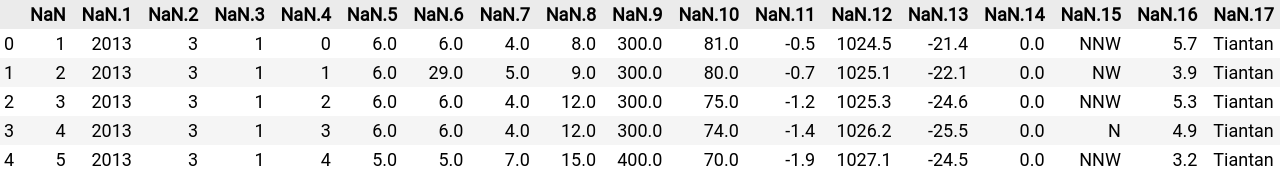
\includegraphics[width=\linewidth,height=2.7cm]{head_before_rename.png}
    \caption{output del metodo head prima della rinomina delle colonne}
    \label{fig:head_before_rename}
\end{figure}
Come si può notare nell'immagine~\ref*{fig:head_before_rename} i nomi delle colonne 
non hanno nessun nome significativo, con il seguente esempio potremmo
cambiare il nome delle colonne.

\paragraph{Snippet}
\begin{minted}{python3}
    # definizione di una lista di nomi per le colonne del dataset
    dataset.columns = [ 'no',    'year',  'month', 'day', 'hour', 
                        'pm2_5', 'pm10',  'so2',   'no2', 'co',  
                        'o3',    'temp',  'pres',  'dewp','rain',  
                        'wd',    'wspm',  'station']
    display(dataset.head())
\end{minted}
\begin{figure}[h!]
    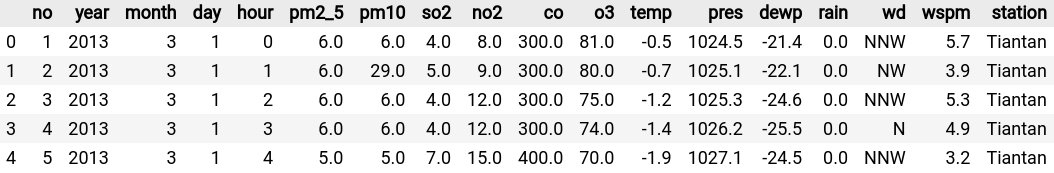
\includegraphics[width=\linewidth,height=2.7cm]{head_after_rename.png}
    \caption{output del metodo head dopo la rinomina delle colonne}
    \label{fig:head_after_rename}
\end{figure}
Come si può notare nell'immagine~\ref*{fig:head_after_rename}
assegnando la lista delle colonne come attuali nomi per le serie del dataset
riusciamo ad ottenere un'interpretazione più accurata.


\subsubsection{Scelta dell'indice}
Molte delle funzionalità fornite da \texttt{pandas} ed altri pacchetti python
richiedono che il dataset sia indicizzato nel tempo nel corretto modo.
In figura~\ref*{fig:head_after_rename} si può notare che la prima colonna
senza nome e la seconda colonna con nome \texttt{no}, indichino
il numero di riga per ogni misurazione, la differenza è che la prima colonna
è generata automaticamente dal pacchetto \texttt{pandas}, ed impostata
di default come indice, mentre la seconda con
nome \texttt{no} è fornita direttamente dal file csv precedentemente caricato.
Per l'analisi della maggior parte delle serie temporali un'idicizzazione per numero
di riga non è significativa, sarebbe molto più conveniente lavorare avendo
come indice di tabella la data ed ora di ogni effettiva misurazione.
A questo proposito il dataset caricato ci fornisce delle colonne (\texttt{year}
, \texttt{month}, \texttt{day} e \texttt{hour}) indicizzate per tempo e relative
ad ogni misurazione, che possono essere riformattate insieme ed usate come indice
per il dataset.

\paragraph{Snippet}
\begin{minted}{python3}
    # unificazione delle colonne relative al tempo per ogni 
    # istante di tempo t in una nuova colonna
    new_index_column = []
    for i in range(len(dataset.year)):
    new_index_column.append("%s/%s/%s %s:0:0" 
        % (dataset.day[i], dataset.month[i], 
           dataset.year[i], dataset.hour[i]) )

    # elimina le colonne relative al tempo
    del dataset["year"], dataset["month"], 
        dataset["day"], dataset["hour"], 
        dataset["no"]

    # imposta/crea la nuova colonna date e converti in datetime
    dataset['date'] = new_index_column
    dataset['date'] = pd.to_datetime(dataset.date, dayfirst=True)

    # imposta come index la nuova colonna date
    dataset.set_index("date", inplace=True)
    display(dataset.head())
\end{minted}
\begin{figure}[h!]
    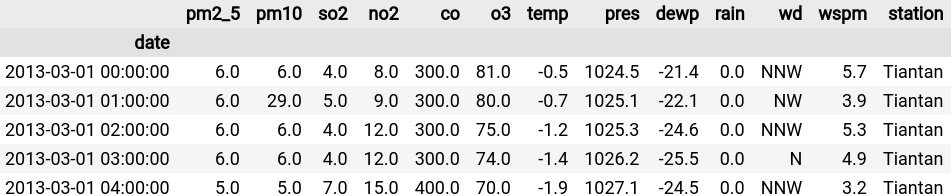
\includegraphics[width=\linewidth,height=2.7cm]{head_after_index_set.png}
    \caption{output del metodo head dopo aver impostato l'indice}
    \label{fig:head_after_index_set}
\end{figure}
Come si può notare dall'output del metodo \texttt{head} nell'immagine \ref*{fig:head_after_index_set}
\texttt{date} è stato impostato come indice di tabella e quindi da questo momento in poi
possiamo accedere al dataset, scegliendo le misurazioni interessate, utilizzando la
data.

\paragraph{Periodo di campionamento}
Un'altra importante modifica è impostare il periodo di campionamento del dataset,
in poche parole impostare un corretto indice non basta a massimizzare il corretto
funzionamento delle funzionalità di analisi delle serie temporali, bisogna anche specificare
l'istante di tempo che occorre tra una misurazione e l'altra. Per fare ciò
\texttt{pandas} fornise un metodo che imposta il periodo di campionamento
a quello deiderato, nel nostro caso sappiamo che le misurazioni sono state campionate
ogni ora.
\subparagraph{Snippet}
\begin{minted}{python3}
    # imposta il periodo di capionamento 
    # del dataset ad ogni ora
    dataset = dataset.asfreq("h")
\end{minted}

\subsubsection{Individuazione dei valori nulli e possibili soluzioni}
La presenza di valori nulli in una serie può avere molteplici cause, ad esempio,
l'impossibilità da parte dello strumento di capionare ad un certo istante di tempo $t$,
oppure se pensiamo ad una fotocamera che acquisisce delle coordinate relative ad un soggeto,
l'uscita di esso dall'obbiettivo.

Indifferentemente dal motivo per cui dei valori nulli sono presenti, 
in una serie o un dataset, la loro presenza può causare molti
problemi sia nel corretto funzionamento di alcune funzionalità per l'analisi sia perchè
non avere dei valori in determinati punti della serie, in certe applicazioni, potrebbe
essere un problema. \texttt{pandas} fornisce dei metodi utili, e semplici, alla soluzione di questo
problema ma ovviamente ogni problema è diverso e quindi, per applicazioni specifiche,
potrebbe essere necessario cercare soluzioni differenti. In questa sezione ci limitiamo
a descrivere le funzionalità fornite da \texttt{pandas} per la soluzione a questo problema.

\paragraph{Controllo}
Per controllare la presenza di valori nulli \texttt{pandas} fornisce un metodo chiamato
\texttt{isna} che ritorna un dataset dove, per ogni misurazione, indica \texttt{True}
se la misurazione è \texttt{NaN} altrimenti \texttt{False}. Sommando i valori \texttt{True}
per ogni colonna possiamo controllare quanti valori nulli sono presenti per ogni serie.\\
\\
\subparagraph*{Snippet}
\begin{minted}{python3}
    # controllo valori nulli
    dataset.isna().sum()
\end{minted}
\begin{figure}[h!]
    \centering
    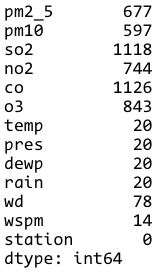
\includegraphics[width=0.24\linewidth,height=5cm]{somma_valori_nulli.png}
    \caption{output della somma dei valori nulli relativi ad ogni serie del dataset}
    \label{fig:sum_null}
\end{figure}
Come si puo notare dall'output del comando in figura~\ref*{fig:sum_null}
il nostro dataset contiene molteplici valori nulli, ora vediamo come poter risolvere
il segente problema

\paragraph{Back fill o Forward fill}
\texttt{pandas} fornisce la possibilità di ``riempire'' i valori nulli in due diverse
modalità tramite l'utilizzo del metodo \texttt{fillna}
\begin{itemize}
    \item \textbf{Back fill}: permette di sostituire i valori nulli con la succesiva
    misurazione valida.
    \item \textbf{Forward fill}:  permette di sostituire i valori nulli propagando
    l'ultima valida misurazione alla prossima valida.
\end{itemize}
Entrambi i metodi gestiscono i valori nulli più o meno nella stessa maniera ma la scelta
di uno piuttosto che l'altro cambia da caso in caso dipendendtemente dal risultato
ottenuto dopo l'utilizzo di essi.


Per i nostri esempi il risulato nell'utilizzo di un metodo piuttosto che l'altro
portava comunque ad un risultato soddisfacente.\\
\\
\subparagraph*{Snippet}
\begin{minted}{python3}
    # rimepimento dei valori nulli 
    # mediante il metodo di forward fill
    dataset = dataset.fillna(method="ffill")
    dataset.isna().sum()
\end{minted}
\begin{figure}[h!]
    \centering
    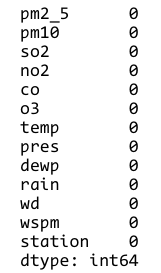
\includegraphics[width=0.24\linewidth,height=5cm]{somma_valori_nulli_dopo_fill.png}
    \caption{output della somma dei valori nulli relativi ad ogni serie del dataset dopo l'utilizzo del metodo \texttt{fillna}.}
\end{figure}


\paragraph{Interpolazione} 
Un possibile metodo, non fornito dalle funzionalità del pacchetto \texttt{pandas},
che potrebbe essere utilizzato è quello di interpolare i dati così da poter colmare
i vuoti creati dai valori nulli. Questa funzionalità non è stata sviluppata
in quanto non fine allo scopo di questo tirocinio ma, in certe applicazioni, si potrebbe
voler utilizzare una metodologia basata su questa tecnica per ottenere una rappresentazione
più accurata dei dati.


\paragraph{Altro metodo non convenzionale}
Un altro metodo non convenzionale, non presente tra le funzionalità fornite,
è quello di poter eliminare i valori nulli dalle serie semplicemente
eliminandoli. Ovviamente questo concetto di eliminare una misurazione nulla va
contro a tutte le premesse fatte fino ad ora, non avendo così una ``reale''
serie temporale poichè mancherebbe una misurazione ad un determinato istante di tempo
$t$, e molte delle analisi che si vorrebbero poter fare su una serie risulterebbero
inapplicabili. 
Tuttavia, in qualche applicazione particolare (come vedremo in seguito), una funzionalità
che semplicemente elimina i valori nulli da una serie potrebbe tornare comoda.
\subparagraph*{Snippet}
\begin{minted}{python3}
    import math as math # import del pacchetto math

    def delete_nan(series: pd.Series | list):
    """ emlimina i valori nulla da una serie
    """
    new_series = []
    for idx, value in enumerate(series):
        if not math.isnan(value):
            new_series.append(value)
    return np.array(new_series)
\end{minted}


\subsubsection{Filtraggio}
Nella maggior parte dei casi quando si parla di serie temporali fonite direttamente 
da apparecchiature che eseguono le misurazioni, i dati si presentano in maniera
``grezza'' ed è quindi necessario filtrarli per poter rimuovere una buona parte
del rumore presente. Questo passaggio è molto importante se parliamo di dati non elaborati
in quanto avere del rumore in una serie temporale o, più in generale, in qualsiasi
tipo di segnale, porta a leggere delle misurazioni ``false''. Solitamente il rumore
indesiderato risiede nelle frequenze alte del segnale, quindi, a questo proposito,
vediamo come poter filtrare una sorgente ``grezza'' di dati mediante l'utilizzo del
modulo \texttt{signal} del pacchetto \texttt{scipy}.

\paragraph{Filtro di Butterworth}
Per poter rimuovere una buona parte del rumore, come scelta generale, in questo tirocinio,
si è utilizzato il filtro di Butterworth che permette di regolare parametri come la 
frequenza di taglio e l'inclinazione (slope) della curva di taglio.

\begin{figure}[H]
    \centering
    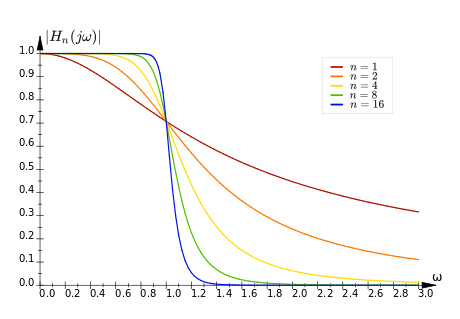
\includegraphics[width=0.7\linewidth,keepaspectratio]{butterworth_filter.png}
    \caption{Filtro di Butterworth normalizzato.}
    \label{fig:butterworth_filter}
\end{figure}

Per poter apprezzare la differenza tra un segnale filtrato da un segnale ``grezzo''
seguirà un esempio su come questo filtro possa essere applicato tramite l'utilizzo
delle funzionalià fornite dal modulo precedentemente citato.

\begin{esempio} [Utilizzo del filtro di Butterworth]
Consideriamo un segnale la cui distanza tra ogni misurazione è di $\frac{1}{30}$
di secondo, presenta una frequenza di campionamento di $30\mathsf{Hz}$.

\begin{figure}[H]
    \centering
    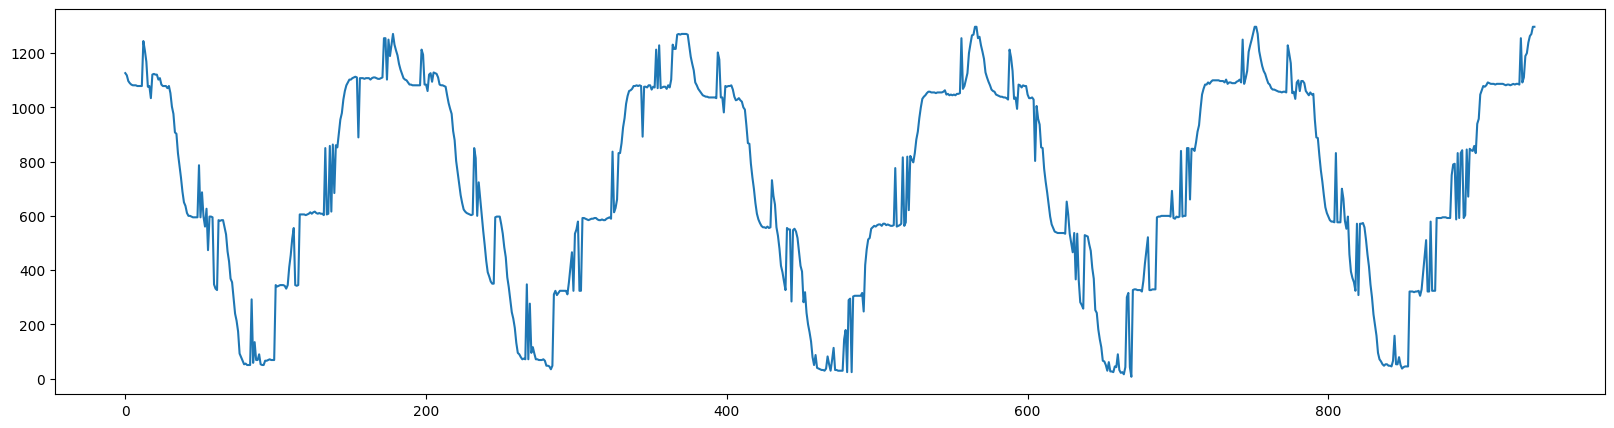
\includegraphics[width=\linewidth,height=4.2cm]{segnale_non_filtrato.png}
    \caption{Segnale non filtrato.}
    \label{fig:segnale_non_filtrato}
\end{figure}

In figura~\ref*{fig:segnale_non_filtrato} possiamo notare come nel segnale
in questione sia presente parecchio rumore, facilmente visibile da tutti i picchi 
presenti nel grafico. Proviamo ad applicare il filtro di Butterworth con una frequenza
di taglio sulle $2\mathsf{Hz}$ ed un'inclinazione della curva di taglio di $5$, lasciando
così passare le basse frequenze.


\paragraph{Snippet}
\begin{minted}{python3}
    # slope/inclinazione della curva di taglio
    inclinazione = 5 

    # frequenza di taglio
    frequenza_taglio = 2

    # frequenza di campionamento
    frequenza_di_campionamento = 30

    # creazizone del filtro di Butterworth
    b, a = signal.butter(inclinazione, 
                        frequenza_taglio, 
                        fs=frequenza_di_campionamento)

    # applicazione del filtro sul segnale
    segnale_filtrato = signal.filtfilt(b, a, series)
\end{minted}

\begin{figure}[H]
    \centering
    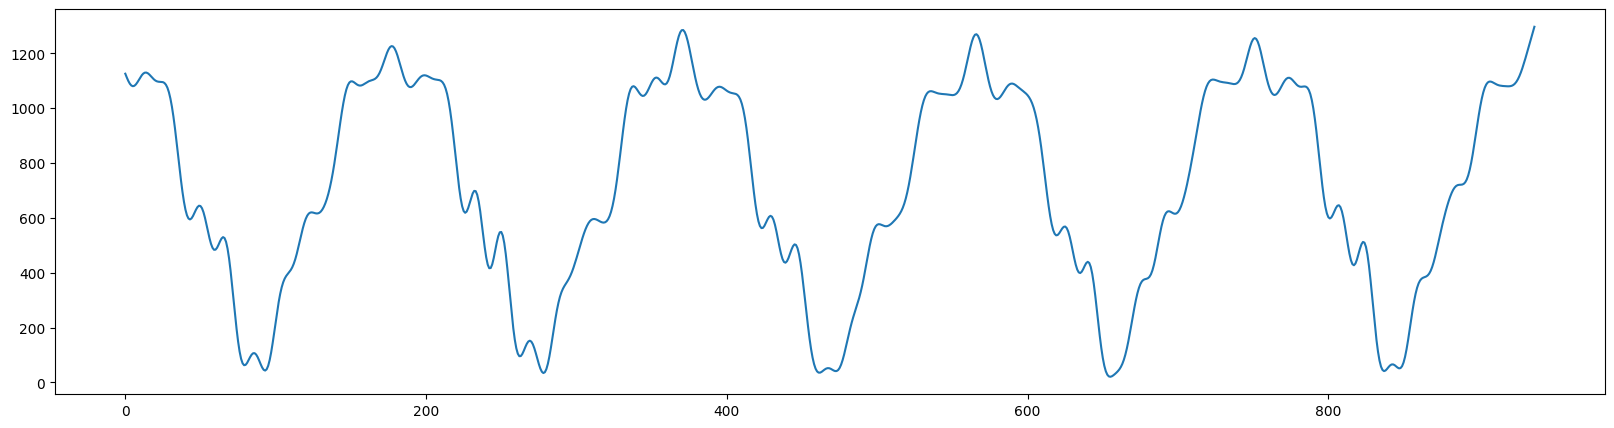
\includegraphics[width=\linewidth,height=4.2cm]{segnale_filtrato.png}
    \caption{Segnale filtrato.}
    \label{fig:segnale_filtrato}
\end{figure}

In figura~\ref*{fig:segnale_filtrato} viene rappresentato il segnale dopo l'applicazione
del filtro passa basse di Butterworth, come si può notare una buona parte del rumore
non è più presente e non avendo i picchi presentati nella sua versione non filtrata.

\end{esempio}


\paragraph{Scelta dei parametri e del filtro}
Dipendendtemente dal tipo di filtraggio che si vuole ottenere conviene applicare un 
filtro piuttosto che un altro e la sua relativa scelta dei parametri cambia da
applicazione ad applicazione e dal tipo di risultato che si vuole ottenere.


    \subsection{Componenti di una serie temporale}
In questo sottocapitolo ci soffermeremo a spiegare le componenti principali
che compongono una serie temporale per poterne analizzare l'andamento e/o
eventuali pattern ricorrenti.


Molte volte è utile suddividere una serie temporale in più diverse componenti
distinte per poterne analizzare singolarmente il loro comportamento e quindi successivamente
riuscire ad inferire sul generale andamento della serie. Possiamo quindi
pensare ad una serie temporale come un insieme di 3 componenti principali:
Trend (andamento/tendenza), Stagionalità e Residui (più comunemente detta Noise).

\subsubsection{Trend}
La componente di trend è un pattern nei dati che mostra che mostra il 
movimento (andamento) di una serie verso valori relativamente più alti o più bassi 
in un lungo periodo di tempo. In altre parole, il trend si osserva quando 
la serie temporale presenta una pendenza crescente o decrescente. 
La tendenza di solito si verifica per un certo periodo di tempo 
e poi scompare, non si ripete. Ad esempio, una nuova canzone, 
che diventa di tendenza per un po' di tempo e poi scompare. 
Non c'è alcuna possibilità che torni in tendenza~\cite{gg:trend}.


Il trend potrebbe essere:
\begin{itemize}
    \setlength\itemsep{-0.6em}
    \item \textbf{Uptrend}: L'analisi delle serie temporali mostra un andamento generale al rialzo, quindi si tratta di Uptrend.
    \item \textbf{Downtrend}: L'analisi delle serie temporali mostra un andamento al ribasso, quindi si tratta di un downtrend.
    \item \textbf{Trend orizzontale o stazionario}: Se non si osserva alcun pattern, si parla di trend orizzontale o stazionario.
\end{itemize}

Se pensiamo al trend come ad una retta, essa sarà la retta che meglio approssima i dati. Se 
la retta ha coefficiente angolare positivo allora essa mostrerà un andamento generale al rialzo,
se ha coefficiente angolare negativo allora essa mostrerà un andamento generale al ribasso, mentre se
avrà coefficiente angolare uguale a $0$ non si osserverà alcun pattern.
Ovviamente nella realtà non sempre una retta basta ad avere una buona approssimazione dei dati, quindi
esistono anche altri tipi di trend come il trend esponenziale.

Nella pratica dell'analisi delle serie temporali in python il trend viene stimato mediante 
l'utilizzo di una funzione chiamata \textit{moving average} (trattata in una sezione successiva).

\begin{esempio} [esempio pratico di trend]
    Consideriamo come serie temporale una serie la cui per ogni osservazione abbiamo
    la temperatura media giornaliera nella città di Beijing a partire 
    dal $01/01/2013$ al $01/01/2017$.

    \begin{figure}[H]
        \centering
        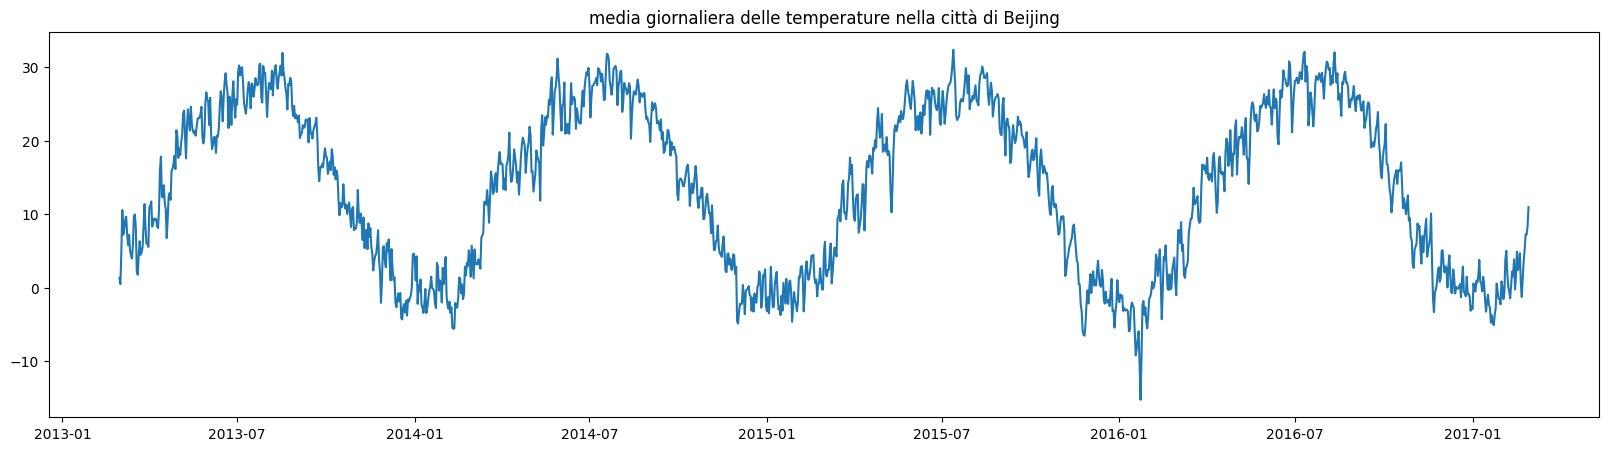
\includegraphics[width=\linewidth,height=4.7cm]{media_giornaliera_temp.png}
        \caption{Grafico della temperatura media giornaliera nella città di Beijing.}
        \label{fig:media_giornaliera_temp}
    \end{figure}

    Consideriamo ora un periodo di un anno ($365$ giorni) il trend avrà un grafico
    come il seguente

    \begin{figure}[H]
        \centering
        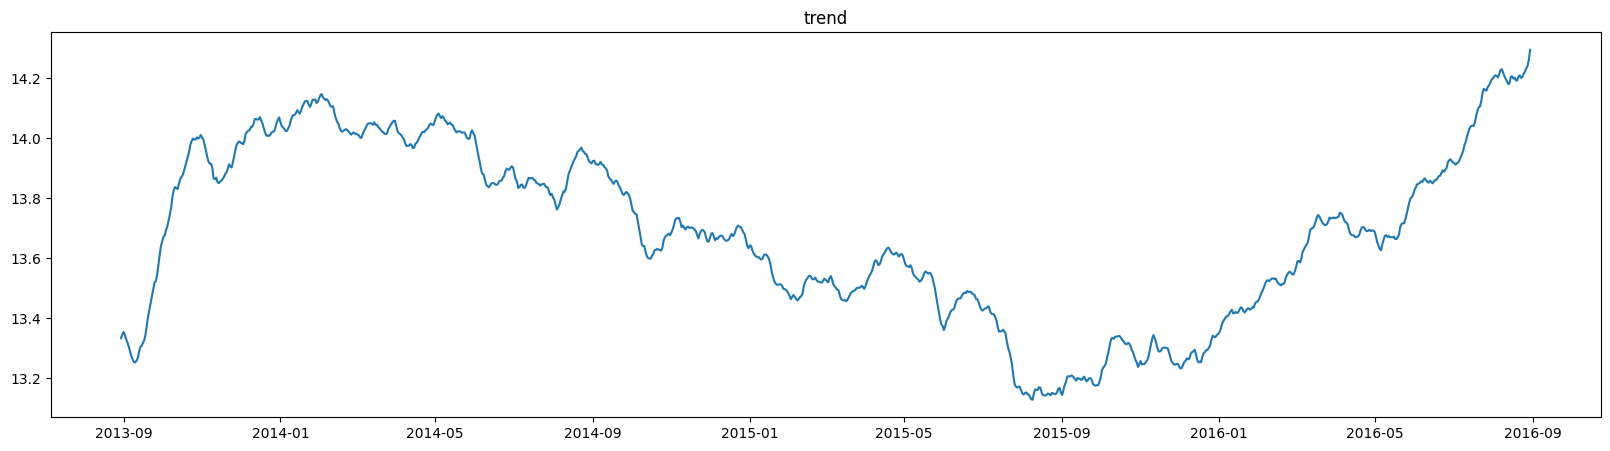
\includegraphics[width=\linewidth,height=4.7cm]{media_giornaliera_temp_trend.png}
        \caption{Trend della serie in figura~\ref{fig:media_giornaliera_temp}.}
        \label{fig:media_giornaliera_temp_trend}
    \end{figure}

    Come possiamo vedere dal grafico in figura~\ref{fig:media_giornaliera_temp_trend} 
    il trend viene stimato utilizzando la media dei precedenti $365$ giorni, ovviamente
    la scelta del periodo su cui stimare il trend influisce direttamente sul grafico. 

\end{esempio}


\subsubsection{Stagionalità}
La stagionalità è un aspetto cruciale dell'analisi delle serie temporali. 
Poiché le serie temporali sono indicizzate in avanti nel tempo, sono soggette a 
fluttuazioni stagionali. Ad esempio, ci aspettiamo che le vendite di gelati siano 
maggiori nei mesi estivi e minori in quelli invernali.

La stagionalità può manifestarsi in diversi intervalli di tempo, 
come giorni, settimane o mesi. La chiave per l'analisi delle serie temporali 
è capire come la stagionalità influisce sulle nostre serie~\cite{md:seasonality}.

In sintesi possiamo quindi pensare alla stagionalità come un pattern che si ripete ad 
intervalli/periodi specifici nel tempo.


\begin{esempio} [esempio pratico di stagionalità]

    Se consideriamo come serie temporale la stessa serie utilizzata 
    nell'esempio precedente del trend, quindi una serie la cui 
    ogni osservazione indica la temperatura media giornaliera  
    nella città di Beijing a partire dal $01/01/2013$ al $01/01/2017$

    \begin{figure}[H]
        \centering
        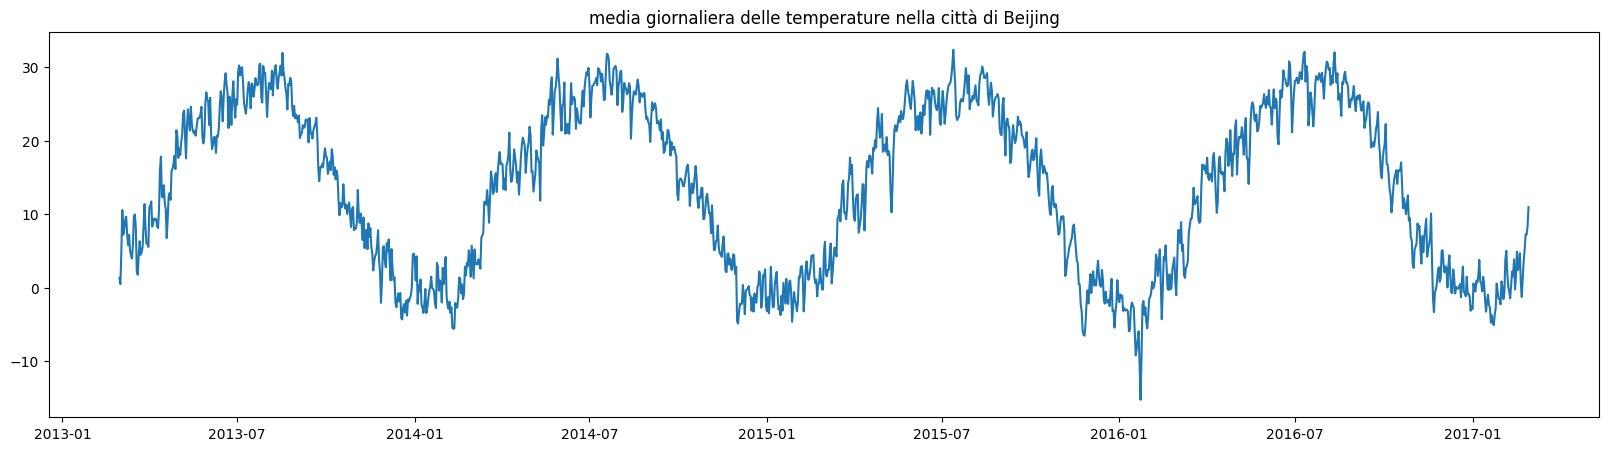
\includegraphics[width=\linewidth,height=4.7cm]{media_giornaliera_temp.png}
        \caption{Grafico della temperatura media giornaliera nella città di Beijing.}
        \label{fig:media_giornaliera_temp2}
    \end{figure}

    e consideriamo un periodo di un anno ($365$ giorni) la stagionalità avrà un grafico
    come il seguente

    \begin{figure}[H]
        \centering
        \includegraphics[width=\linewidth,height=4.7cm]{media_giornaliera_temp_stagionalità.png}
        \caption{Stagionalità del grafico in figura~\ref{fig:media_giornaliera_temp2}.}
        \label{fig:media_giornaliera_temp_stag}
    \end{figure}

    Il grafico in figura~\ref{fig:media_giornaliera_temp_stag} rappresenta la stagionalità
    della serie rappresentata in figura~\ref{fig:media_giornaliera_temp2}.
    Se guardiamo con occhio attento il grafico della stagionalità, possiamo notare come
    ad intervalli di un anno esso si ripeta, creando così il pattern stagionale.

\end{esempio}


\subsubsection{Residui}
La componente di residui, o più comunemente detta noise, può essere considerata come
la parte restante tra il trend e la stagionalità, quindi una sorta di errore.

Un metodo per poter capire meglio come rappresenta la componente di residui 
è considerare, ad esempio, una serie temporale con trend orizzontale e nessun pattern
stagionale, ed applicare la definizione di residui, quindi tutto quello che rimane
tolto il trend e la stagionalità.

\begin{esempio} [esempio pratico di stagionalità]

    Se consideriamo la serie temporale utilizzata negli esempi del trend
    e della stagionalità, la componente dei residui avrà un grafico come il seguente

    \begin{figure}[H]
        \centering
        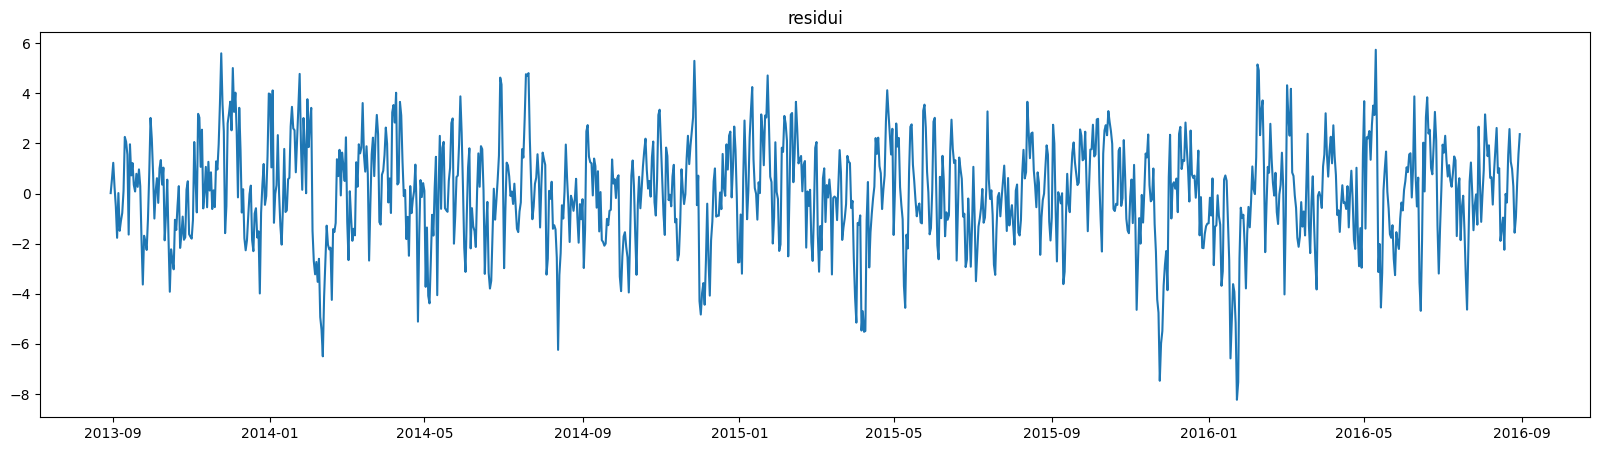
\includegraphics[width=\linewidth,height=4cm]{media_giornaliera_temp_residui.png}
        \caption{Residui della media giornaliera delle temperature nella città di Beijing.}
    \end{figure}

\end{esempio}


\subsubsection{Decomposizione di una serie}
Esistono due modalità distinte per la decomposizione di
una serie temporale nelle sue 3 componenti principali. La prima modalità è detta
additiva in cui le componenti vengono semplicemente sommate, mentre la seconda
è detta moltiplicativa dove le componenti, come suggerisce il termine, 
vengono moltiplicate.

\paragraph{Decomposizione additiva} 
Una decomposizione additiva consiste nella
somma delle componenti. Se consideriamo una serie temporale ad un 
istante $t$ allora essa sarà composta da
\[ y_t = S_t + T_t + R_t \]
dove $y_t$ è l'osservazione, $S_t$ è la componente di stagionalità, 
$T_t$ è la componente di Trend ed $R_t$ è la componente dei residui, tutti
all'istante di tempo $t$.
\begin{figure}[H]
    \centering
    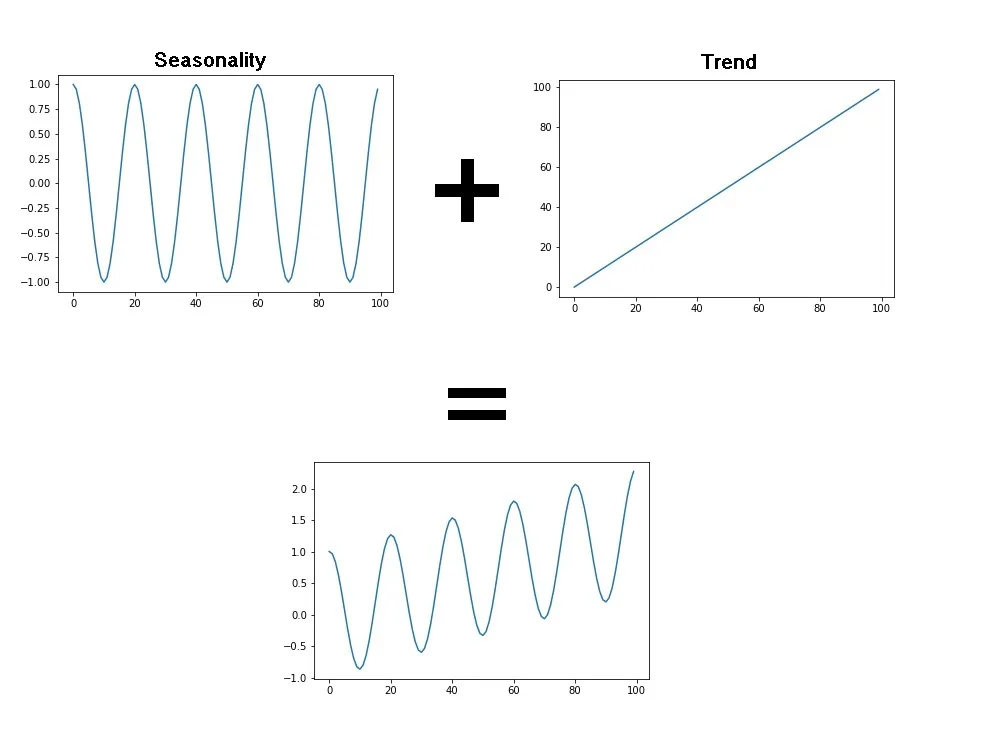
\includegraphics[width=0.6\linewidth]{additive_decomposition.jpg}
    \caption{Decomposizione additiva (escluso residui). [ref imag~\cite{md:seas_dec_imags}]}
    \label{fig:dec_serie_add}
\end{figure}


\paragraph{Decomposizione moltiplicativa} 
Una decomposizione moltiplicativa consiste nella
moltiplicazione delle componenti. Se consideriamo una serie temporale ad un 
istante $t$ allora essa sarà composta da
\[ y_t = S_t \times T_t \times R_t \]
dove $y_t$ è l'osservazione, $S_t$ è la componente di stagionalità, 
$T_t$ è la componente di Trend ed $R_t$ è la componente dei residui, tutti
all'istante di tempo $t$.
\begin{figure}[H]
    \centering
    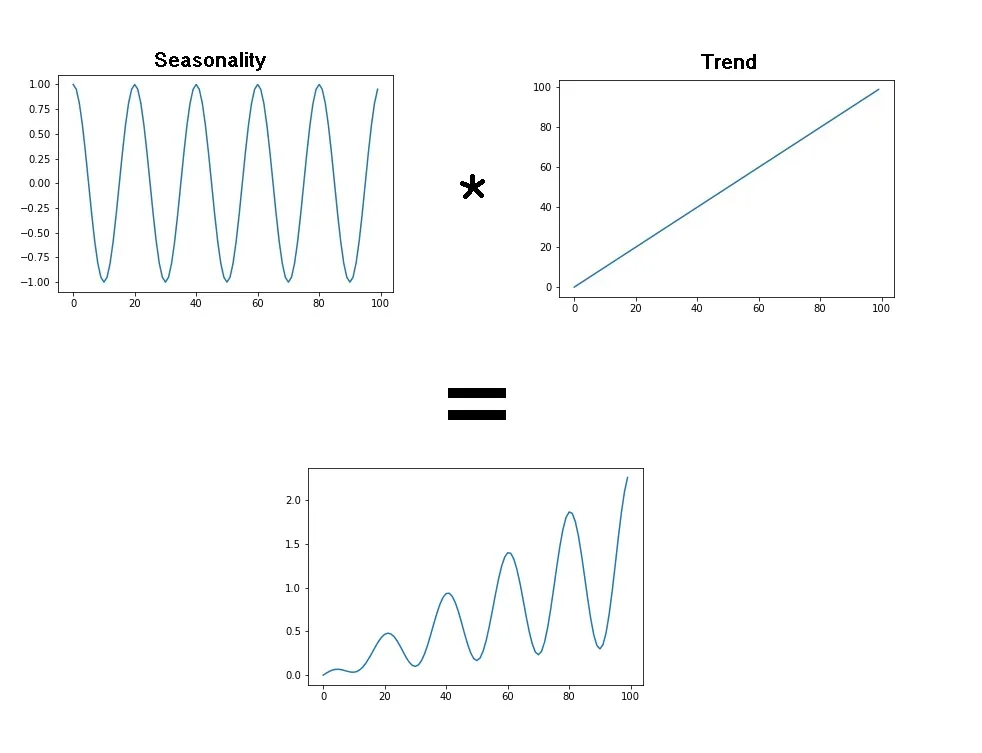
\includegraphics[width=0.6\linewidth]{multiplicative_decomposition.jpg}
    \caption{Decomposizione moltiplicativa (escluso residui). [ref imag~\cite{md:seas_dec_imags}]}
    \label{fig:dec_serie_mul}
\end{figure}

\paragraph{Scelta della modalità di decomposizione}
La scelta della modalità di decomposizione di una serie temporale è importate poiché
la sua decomposizione potrebbe apparire insensata scelta la modalità sbagliata.
Una decomposizione additiva è principalmente appropriata se il magnitudo della 
stagionalità non varia con il livello della serie temporale mentre se, la variazione
della componente di stagionalità, appare proporzionale al livello della serie una modalità
moltiplicativa potrebbe essere più appropriata (per capire la seguente frase guarda le figure
~\ref{fig:dec_serie_add} e~\ref{fig:dec_serie_mul}).


\paragraph{Decomposizione in python}
Vediamo ora come poter decomporre una serie temporale utilizzando la funzione 
\texttt{seasonal\_decompose} fornita dalle funzionalità del pacchetto \texttt{statsmodels}.
\subparagraph*{Installazione del pacchetto}
\begin{minted}{bash}
    pip install statsmodels



\end{minted}

\subparagraph*{Snippet}
\begin{minted}{python3}
    # import del pacchetto 
    from statsmodels.tsa.seasonal import seasonal_decompose

    # periodo utilizzato per il calcolo di trend e stagionalità
    periodo = 365 

    # decomposizione della serie
    decomposition = seasonal_decompose(serie, period=periodo)

    trend   = decomposition.trend     # trend
    stag    = decomposition.seasonal  # stagionalità
    residui = decomposition.resid     # residui
\end{minted}
    \subsection{Stazionarietà}


\subsubsection{Dickey Fuller Test}
    \subsection{Smoothing}

\subsubsection{Moving average}

\subsubsection{Exponential}

\subsubsection{Double Exponential}
    \subsection{Autocorrelazione ed Autocorrelazione parziale}
In questa sezione verranno presentate le funzioni di autocorrelazione ed autocorrelazione
parziale utilizzate nell'analisi di serie temporali per poter trovare pattern e la correlazione
diretta o indiretta della serie con una sua versione spostata lungo l'asse temporale.

Nota che per molte applicazioni (come l'analisi di pattern) che utilizzano le funzioni
di autocorrelazione ed autocorrelazione parziale, le serie temporali devono essere stazionarie.

\subsubsection{Funzione di Autocorrelazione}
L'autocorrelazione definisce il grado di dipendenza tra i valori assunti 
da una funzione campionata nel suo dominio in ascissa. \\
Se è dimostrata l'autocorrelazione tra due valori, al cambiare delle peculiarità 
di uno di essi varierà anche l'altro.

L'autocorrelazione è uno strumento matematico usato frequentemente nella teoria dei 
segnali per l'analisi di funzioni o di serie di valori. Essa è la correlazione 
del segnale (o più in generale del valore di una variabile) con se stesso; 
in altre parole il segnale all'istante di tempo $t$ viene confrontato con un altro valore 
di se stesso ritardato di una quantità 
$\tau$  (senza tale ritardo il segnale è logicamente sempre uguale) 
per verificare quanto si somigli (più precisamente quanto si correli) 
all'avanzare del tempo. Possiamo dedurre che se un segnale varia lentamente nel tempo, 
il valore degli istanti $y(t)$ e $y(t + \tau)$ sarà pressoché simile 
(l'autocorrelazione avrà segno positivo), mentre se varia rapidamente, 
il valore di tali istanti sarà molto diverso e l'autocorrelazione assume 
un valore prossimo allo zero. 
L'autocorrelazione si utilizza spesso per cercare porzioni periodiche che si ripetono 
all'interno di un segnale, in modo tale da determinare la presenza di un segnale 
periodico che è stato sepolto da un rumore, o identificare la frequenza fondamentale 
di un segnale~\cite{wiki:autcor_it}.

Informalmente, è la somiglianza tra le osservazioni di una variabile casuale 
in funzione dell'intervallo di tempo che le separa~\cite{wiki:autcor_en}.

\paragraph{Definizione matematica} 
\subparagraph*{Caso continuo}
Dato un segnale $f(t)$ continuo ed indicizzato nel tempo, l'autocorrelazione $R_{ff}(\tau)$
è definita come la cross-correlazione di $f(t)$ con se stesso avente un ritardo di $\tau$
\[R_{ff}(\tau) = \int_{-\infty}^{\infty} f(t+\tau) \overline{f(t)}  \,dt =  \int_{-\infty}^{\infty} f(t) \overline{f(t-\tau)}  \,dt \]
dove $\overline{f(t)}$ indica il complesso coniugato fi $f(t)$. 
Nota come il parametro $t$ nell'integrale è una variabile fittizia ed è solo necessaria
a calcolare l'integrale. Non ha un significato specifico~\cite{wiki:autcor_en}.

\subparagraph*{Caso discreto}
Nel caso discreto la funzione di autocorrelazione è definita come:
\[ R_{ff}(\tau) = \mathbb{E} \left[ f(t) \overline{f(t-\tau)} \right] = \mathbb{E} \left[ f(t + \tau) \overline{f(t)} \right] \] 

\subparagraph*{Normalizzazione del caso discreto}
La normalizzazione della funzione di autocorrelazione nel caso discreto ci fornisce la 
possibilità di avere una visualizzazione con valori compresi tra $[-1, 1]$. 
Sottraendo la media prima della moltiplicazione si ottiene la funzione di autocovarianza 
\[ 
K_{ff}(\tau) = 
\mathbb{E} \left[ \left( f(t + \tau) - \mu \right) \overline{ \left( f(t) - \mu \right) } \right] =  
\mathbb{E} \left[ f(t + \tau) \overline{ f(t) } \right] - \mu\overline{\mu} 
\] 
dove $\mu$ è la media.


La funzione di autocorrelazione normalizzata viene definita come 

\[ 
\rho_{ff}(\tau) = \frac{K_{ff}(\tau)}{\sigma^2} = 
\frac{\mathbb{E} \left[ \left( f(t + \tau) - \mu \right) \overline{ \left( f(t) - \mu \right) } \right]}{\sigma^2}
\] 



\paragraph{Implementazione della funzione di autocorrelazione ed esempi}
Vediamo ora come poter implementare la funzione di autocorrelazione (normalizzata).
\subparagraph*{Snippet} (\textit{shift di una funzione})
\begin{minted}{python3}
def shift(X, n):
    """ Shifta di n periodi la funzione X
    """


    # controllo per n
    if not isinstance(n, int):
        raise Exception('n deve essere un valore intero')

    X_copy = X.copy() # copia e rendi numpy array
    if not isinstance(X_copy, np.ndarray):
        X_copy = np.array(X_copy)

    # se si shifta troppo impostiamo n
    # alla lunghezza della funzione X
    if np.abs(n) > len(X):
        n = np.sign(n) * len(X)
    
    # dato  n shiftiamo la funzione verso sinistra
    # dato -n shiftiamo la funzione verso destra
    for i in range(np.abs(n)):
        # togliamo il primo o lultimo valore
        # in base a dove vogliamo shiftare
        X_copy = X_copy[1:] if np.sign(n) == 1 else X_copy[:-1]

        # shifta la funzione aggiungendo uno 
        # 0 in testa o in coda in base a dove
        # vogliamo shiftare
        X_copy = np.insert(X_copy, 0 if np.sign(n) == -1 
            else len(X_copy), 0)

    return X_copy.tolist() if not isinstance(X, np.ndarray) \
        else np.array(X_copy)
\end{minted}

\subparagraph*{Snippet} (\textit{singola autocorrelazione})
\begin{minted}{python3}
    def singola_autocorrelazione(X: list | np.ndarray, 
    tau: int, normalizzazione = True) -> float:

    """ Esegue una signola autocorrelazione data la latenza
        tau
    """

    # controllo per tau
    if not isinstance(tau, int) and tau < 0:
        raise Exception('tau deve essere un intero \
            maggiore di 0')

    # controllo che X sia un array numpy
    if not isinstance(X, np.ndarray):
        X = np.array(X)


    if normalizzazione:
        mean = X.mean()
        var = X.var()
        
        # f(t-tau) - mu
        primo_termine   = shift(X - mean, -tau)

        # coniugato(f(t)- mu)
        secondo_termine = np.conjugate(X - mean)

        #                                           ... / sigma^2
        return np.mean( primo_termine * secondo_termine ) / var

    # espettazione[ f(t-tau)       * coniugato(f(t)) ]   
    return np.mean( shift(X, -tau) * np.conjugate(X) )
\end{minted}

\subparagraph*{Snippet} (\textit{funzione di autocorrelazione})
\begin{minted}{python3}
def funzione_autocorrelazione(
    X: list | np.ndarray,
    norm = True
    ) -> list | np.ndarray:
    
    """ calcola la funzione di autocorrelazione
    """
    autocorrelazione: list = []
    # calcola la autocorrelazione singola per ogni
    # possibile tau
    for i in range(len(X)):
        autocorrelazione.append(
            singola_autocorrelazione(X, i, 
                normalizzazione=norm)
        )

    return autocorrelazione if not isinstance(X, np.ndarray) \
        else np.array(autocorrelazione)
\end{minted}

\begin{esempio}[Autocorrelazione]
    Prendiamo come esepio un segnale la cui velocità cambia di ``poco''
    nel tempo.

    \begin{figure}[H]
        \centering
        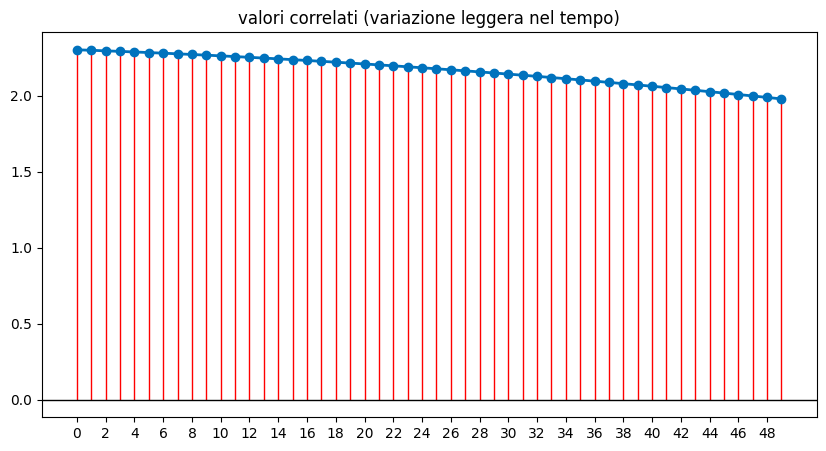
\includegraphics[width=0.9\linewidth,keepaspectratio]{autocor_vel_lenta.png}
        \caption{Autocorrelazione del segnale.}
        \label{fig:autcor_slow}
    \end{figure}

    In figura~\ref{fig:autcor_slow} possiamo notare come l'autocorrelazione non normalizzata
    del segnale varia di poco nel tempo per segnali che variano lentamente.

    Consideriamo ora più segnali la cui velocità cresce velocemente nel tempo.

    \begin{figure}[H]
        \centering
        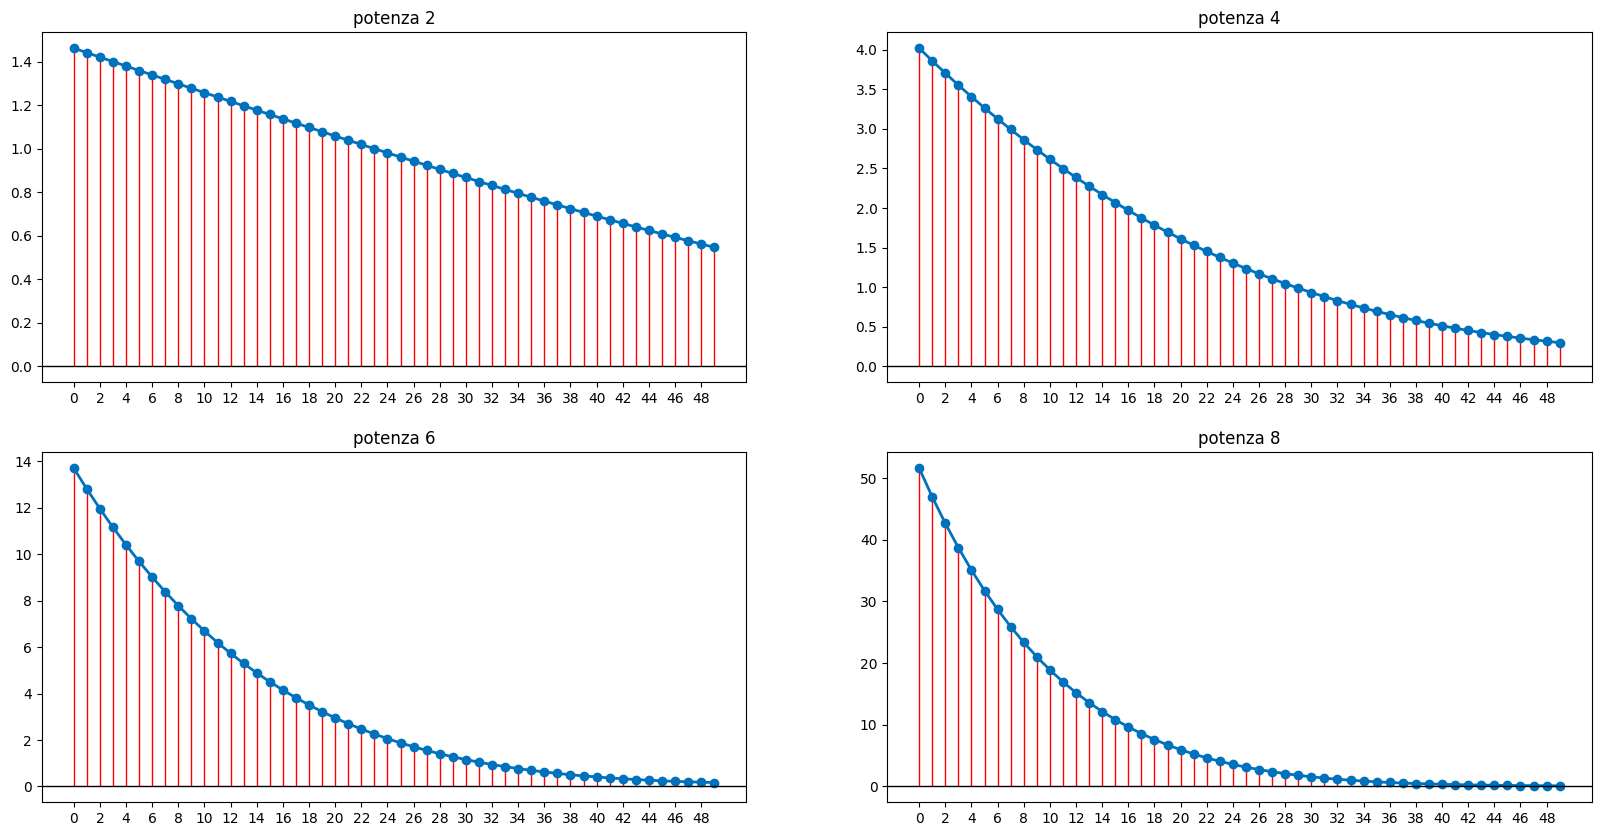
\includegraphics[width=\linewidth,height=9cm]{autocor_vel_fast.png}
        \caption{Autocorrelazione dei segnali.}
        \label{fig:autcor_fast}
    \end{figure}

    In figura~\ref{fig:autcor_fast} possiamo notare come l'autocorrelazione non normalizzata
    dei segnai varia maggiormente nel tempo per segnali che variano velocemente.

    Possiamo quindi osservare come segnali con minima variazione nel tempo avranno anche
    una minima variazione nell'autocorrelazione non normalizzata, mentre segnali che hanno
    un'ampia variazione tra un'osservazione e quella successiva avranno una maggiore variazione 
    anche nell'autocorrelazione non normalizzata.

    Un'ulteriore osservazione che nasce dagli esempi sopra è che i segnali più 
    correlati tra loro sono i segnali con una variazione minore nel tempo, mentre
    i segnali meno correlati saranno i segnali con una maggior variazione. 

\end{esempio}


\subsubsection{Funzione di Autocorrelazione Parziale}
L'autocorrelazione parziale, riassume la relazione tra 
un'osservazione di una serie temporale e le osservazioni di fasi temporali precedenti,
come la normale autocorrelazione con la diversità che le relazioni 
delle osservazioni intermedie vengono rimosse. In sostanza, 
le correlazioni indirette vengono eliminate lasciando visibile solamente
l'effetto diretto~\cite{md:mediumacf_pacf}.

Potreste, ad esempio, essere interessati alla relazione diretta tra i consumi 
di oggi e quelli di un anno fa. Non vi importa nulla di ciò che accade nel mezzo.

Il consumo dei 12 mesi precedenti ha un effetto sul consumo degli 11 mesi precedenti 
e il ciclo continua fino al periodo più recente. Nelle stime di autocorrelazione parziale, 
questi effetti indiretti vengono ignorati~\cite{ain:acf_pacf}.

\paragraph{Calcolo della funzione di autocorrelazione parziale}
La funzione di autocorrelazione parziale teorica di una serie temporale 
stazionaria può essere calcolata utilizzando l'algoritmo di Durbin-Levinson:
\[ \phi_{n,n} = 
\frac
{\rho(n) - \sum_{k = 1}^{n-1}  \phi_{n-1,k}\rho(n-k)}
{1 - \sum_{k = 1}^{n-1} \phi_{n-1,k}\rho(k)} 
\]
    
dove $\phi_{n,k} = \phi_{n-1,k} - \phi_{n,n}\phi_{n-1,n-k}$ per $1 \leq k \leq n-1$ and
$\rho(n)$ è la funzione di autocorrelazione~\cite{wiki:pacf}.

\paragraph{Quando è utile l'autocorrelazione parziale}
La funzione di autocorrelazione parziale gioca un ruolo molto importante, nell'analisi
di serie temporali, per l'identificazione dei lag ``importanti'' per un modello autoregressivo
(AR). Essendo che lo scopo del tirocinio è analizzare 
serie temporali senza eseguire nessuna predizione sui dati con modelli autoregressivi, non verrà
data un'iplementazione della formula presente sopra.

\paragraph{Pacchetto per l'utilizzo}
La funzione \texttt{pacf}, del modulo\\ \texttt{statsmodels.tsa.stattools}, e la funzione
\texttt{plot\_pacf}, del modulo\\ \texttt{statsmodels.graphics.tsaplots}, forniscono rispettivamente
un'implementazione della funzione di autocorrelazione parziale ed il grafico di essa.



    
    % bibliografia
    \section{Bibliografia}
    \printbibliography[title=Bibliografia]

\end{document}  